% 6 - 7  pages
\documentclass[a4paper,twoside]{article}

\usepackage{epsfig}
\usepackage{subfigure}
\usepackage{calc}
\usepackage{amssymb}
\usepackage{amstext}
\usepackage{amsmath}
\usepackage{amsthm}
\usepackage{multicol}
\usepackage{pslatex}
\usepackage{apalike}
\usepackage{SCITEPRESS}     % Please add other packages that you may need BEFORE the SCITEPRESS.sty package.

\subfigtopskip=0pt
\subfigcapskip=0pt
\subfigbottomskip=0pt

\begin{document}

\title{Authors' Instructions: Preparation of Camera-Ready Contributions to SCITEPRESS Proceedings}

\author{\authorname{First Author Name\sup{1}, Second Author Name\sup{1} and Third Author Name\sup{2}}
\affiliation{\sup{1}Institute of Problem Solving, XYZ University, My Street, MyTown, MyCountry}
\affiliation{\sup{2}Department of Computing, Main University, MySecondTown, MyCountry}
\email{\{f\_author, s\_author\}@ips.xyz.edu, t\_author@dc.mu.edu}
}

\keywords{The paper must have at least one keyword. The text must be set to 9-point font size and without the use of bold or italic font style. For more than one keyword, please use a comma as a separator. Keywords must be titlecased.}

\abstract{The abstract should summarize the contents of the paper and should contain at least 70 and at most 200 words. The text must be set to 9-point font size.}

\onecolumn \maketitle \normalsize \vfill

\section{\uppercase{Introduction}}
\label{sec:introduction}

\noindent Accurate sequences classifiacation and subsequences detection are an open problems in different areas of bioinformatics, such as genomics and protenomics. 
Challenge here is a high variability of sequences which one want to mark as a same class.
For some type of sequences its secondary structure is a !!! and this fact may be used for !!!.

For example, algorithms that can efficiently and accurately identify and classify bacterial taxonomic hierarchy have become a focus in computational genetics.
The idea that secondary structure of genomic sequences is sufficient for solving the detection and classification problems lies at the heart of many tools~\cite{GrammarsRNA,PCFG,meta,LWPCFG}. 
The secondary structure can be specified in terms of formal grammars. 
The sequences obtained from the real bacteria usually contain a huge number of mutations and ``noise'' which renders precise methods impractical. 
Probabilistic grammars and covariance models (CMs) are a way to take the noise into account~\cite{EddyDurbin}.
For example, CMs are successfully used in the Infernal tool~\cite{Infernal}.
Neural networks is another way to deal with ``noisy'' data. 
The works~\cite{Humidor,ANN} utilize neural networks for 16s rRNA processing and demonstrate promising results.

In this work we propose the way to combine formal grammars and neural networks for secondary structure features processing.
The key idea is does not try to model full (sub)sequence by grammar, but create grammar which describes features of secondary structure and use neural network for these features processing.

\section{\uppercase{Proposed solution}}
\label{sec:proposedSolution}

\noindent We combine neural networks and ordinary context-free grammars to detect genomic sequences. 
We extract features by using the ordinary (not probabilistic) context-free grammar and use the dense neural network for features processing.
Features can be extracted by any parsing algorithm and then presented as a boolean matrix but we choose parsing algorithm based on matrix multiplication.

\subsection{Context-Free Grammars}

\noindent It is a well-known fact that secondary structure of sequence may be approximated by using formal grammars.
There is number of works that utilize this fact for !!!

The !!! is to use probabilistic grammars.
We use ordinary (not probabilistic) gramars.
Our goal is not to model secondary structure of whall sequence (wich requred probabilistic grammars), but describe features of secondary structure, such as stems, loops, pseudoknots and it's composition.
The set of feature types is limited by class of the grammar which we use.
For example, pseudoknots can not be expressed by context-free grammars, but can be expresed by using cinjunctive~\cite{KanchanDevi2017,zier2013rna,Okhotin:2001:CG:543313.543323} or multiple context-free~\cite{SEKI1991191,Riechert:2016:ADP:2972703.2972851}.

The context-free grammar which we use in our experiments is presented in figue~\ref{fig:cfg-rna}.
More details on it.
Four letters in the alphabet ().
Only calssical base pairs.
\verb|s1| is a stsrt nonterminal.
metarules as a feature of languge.
Stems as an exampl eof metarules usage.

\begin{figure}
\begin{verbatim}
s1: stem<s0> any

a_0_7 : any*[2..10]

s0: a_0_7 | a_0_7 stem<s0> s0

any: A | U | C | G

stem1<s>: A s U | G s C | U s A | C s G 

stem2<s>: stem1< stem1<s> >

stem<s>:  
      A stem<s> U 
    | U stem<s> A 
    | C stem<s> G 
    | G stem<s> C 
    | stem1< stem2<s> >  
 } 
\end{verbatim}
\caption{Context-free grammar for RNA secondary structure features extraction}
\label{fig:cfg-rna}
\end{figure}

For example, one can varay length of unfoldable sequence \verb|a_0_7 : any*[0..10]| or \verb|a_0_7 : any*[1..8]|.
Also one can increase (or decrease for some reason) the minimal height of stem, or add pseudocnotss description in the grammar.

\begin{figure}
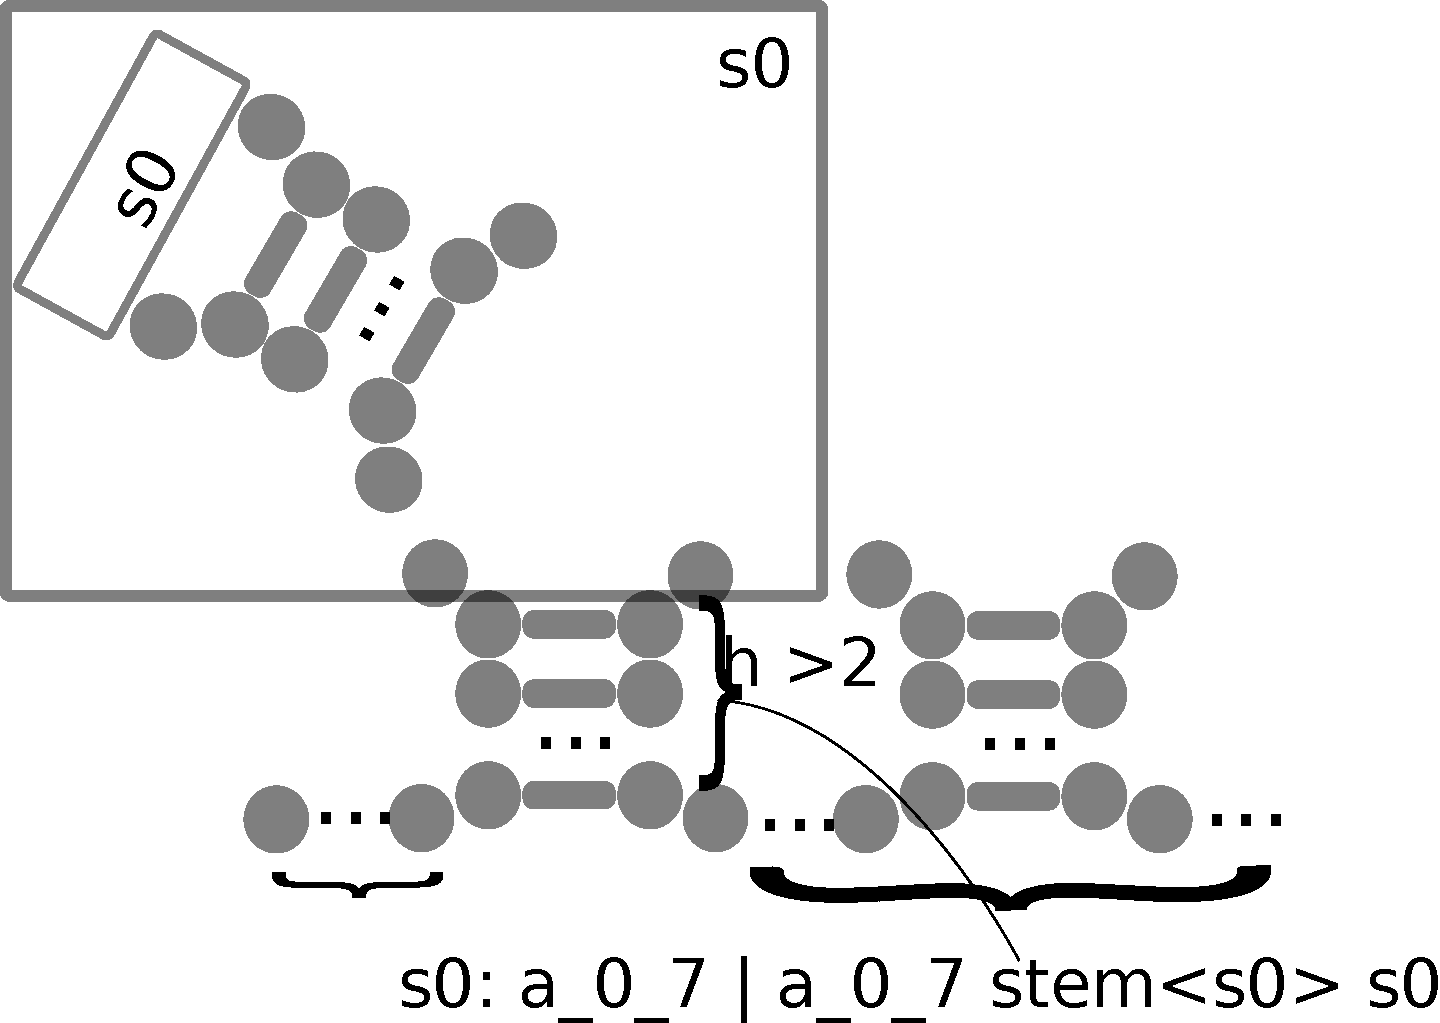
\includegraphics[width=.5\textwidth]{figures/16sgrammar.pdf}
\caption{!!!}
\label{fig:ss}
\end{figure}

\subsection{Parsing Algorithm}

\noindent Parsing is a feature extraction, so undirected parsing: we want to find all derivable substrings of given string for all nonterminals, not to check derivability of given string.

CYK --- as a classical well-known algorithm.

Matrices.

Valiant~\cite{Valiant:1975:GCR:1739932.1740048} --- subcubic algorithm based on matrix multiplication.

Rustam~\cite{Azimov:2018:CPQ:3210259.3210264} --- generalization for graph. Theoretical time complexity is !!! than complexity of the Valiant's algorithm, but in practice these algorithm avoid machnery on submatrices manipulation and demonstarte better performence with simple implementation.

Sparse matrices, boolean, GPGPU, etc.

Matrix-based approach can be generalized to conjunctive and even boolean grammars~\cite{OKHOTIN2014101}, as far as to multiple context-free grammars~\cite{mcfgMatrices}, which can provide a base for more expressive features descriptions handling.

\subsection{Matrices}

\noindent The result of parsing is a set of squere boolean matrices. 
Each matrix $M_N$ contains information of all substrings which can be derived from nontermnal $N$.
In the oter word, $M_N[i,j]=1$ iff $N \Rightarrow^*_G w[i,j]$ where $w$ is the input sequence and $G$ is context-free grammar, and $N$ is a nonterminal.

Detailed description

One matrix for each nonterminal.
We can select nonterminals of interest.


{\centering
  \fbox{
\includegraphics[width=2.5cm]{figures/mt1.png}}
  \
  \fbox{
\includegraphics[width=2.5cm]{figures/mt2.png}}
  \
  \fbox{
\includegraphics[width=2.5cm]{figures/mt3.png}}
  }

Empty triangle can be omitted.
In order to handle matrices by using newral networks we vectorize it.
Row by row.
Complression to int or byte.
It is the reason why we want to try boolean networks.

\subsection{Neural Neworks}

One of possible choice for classificaton.
Classical scenario is to provide features vectors and try to classify them.
In our case ht fact that ``$w[i,j]$ is derivable from nonterminal $N$'' which is encoded in the matrix is a feature.
So, matrix is a set (or vector) of features.

We use dense neural network because locality is broken during vectorisation and any convolutons is inapplicable.

Current architecture and its motivation and explanation.
Huge dropout and batch normalization.

\section{\uppercase{Evaluation}}
\label{sec:evaluation}

\noindent We evaluate the proposed approach for 16s rRNA detection.
We specify context-free grammars which detect stems with the hight of more than two pairs and their arbitrary compositions.
For network training we use dataset consisting of two parts: random subsequences of 16s rRNA sequences from the Green Genes database~\cite{pmid16820507} form positive examples, while the negative examples are random subsequences of full genes from the NCBI database~\cite{pmid19854944}.
All sequences have the length of 512 symbols, totally up to 310000 sequences.
After training, current accuracy is 90\% for validation set (up to 81000 sequences), thus we conclude that our approach is applicable.

\section{\uppercase{Future Work}}
\label{sec:FutureWork}

\noindent The presented is a work in progress. 
The ongoing experiment is finding all instances of 16s rRNA in full genomes.
Also we plan to use the proposed approach for the filtration of chimeric sequences and the classification.
Composition of our approach with other methods and tools as well as grammar tuning and detailed performance evaluation may improve the applicability for the real data processing.


\section{\uppercase{Discussion}}
\label{sec:Discussion}

Protenomics (Witold Dyrka)
More complex grammar: more symbols in alphabet, more complex featres.
More powerful languages required.
One of the possible crutial problem is functionally equivalence sequences with different length in protenomics.

Different lengths. Is a problem.
How can we normalize input?

Construct network which can handle sequences, not parsing data.
It may help to create an embedding.
It may be done by the next way.
\begin{enumerate}
\item Build and train the network which hanle vectorized matricres.
\item Extend this network with head which should convert sequence to !!!
\item Train. Weights of first network is fixed.
\item For concrete problem we can tune weights for full network after second trained to appropriate quality.
\end{enumerate}

Other types of NNs.
Binary, convolutional (try to process matrix as a picture).
Pictures: problem with size, typical matrix size is big.

Prblems with data: how to create balanced set for training.
Datasets (like GreenGenes) contains huge nomder of samples for some well-studied organisms and very small number of samples for other.

Huge amount of experiments in different directions.
Plans should be discussed with community.


\section*{\uppercase{Acknowledgements}}

\noindent The research was supported by the Russian Science Foundation grant 18-11-00100 and a grant from JetBrains Research.


\vfill
\bibliographystyle{apalike}
{\small
\bibliography{example}}


\vfill
\end{document}

